\clearpage
\section{Uveďte formální definici kryptografického systému, symetrické a asymetrické šifry.}

Kryptografický systém pro šifrování zpráv je pětice ($\mathcal{M}$, $\mathcal{C}$, $\mathcal{K}$, $\mathcal{E}$, $\mathcal{D}$), kde
\begin{itemize}
    \item $\mathcal{M}$, je prostor otevřených zpráv
    \item $\mathcal{C}$ prostor šifrovaných zpráv
    \item $\mathcal{K}$ prostor klíčů
    \item $\mathcal{E,D}$ je dvojice zobrazení, která každému klíči \textit{k} $\in \mathcal{K}$ přiřazují transformaci pro zašifrování zpráv \textit{E} a transformaci pro dešifrování zpráv \textit{D}, přičemž pro každé \textit{k} $\in \mathcal{K}$ a \textit{m} $\in \mathcal{M}$ platí \textit{D(k(E(k,m))) = \textit{m}}
\end{itemize}

\textbf{Symetrická šifra} je taková šifra, kde pro každé \textit{k} $\in \mathcal{K}$ lze z transformace zašifrování $E_k$ určit transformaci $D_k$ a naopak.

\textbf{Asymetrická šifra} je taková šifra, kde pro skoro každé \textit{k} $\in \mathcal{K}$ nelze z transformace zašifrování $E_k$ určit transformaci $D_k$ a naopak.
Vhodnou transformací \textit{G} se vygeneruje dvojice parametrů (veřejný a soukromý klíč), kde klíč \textit{k} je tajným nastavením transformace.

\section{Popište, čím se zabývá tzv. „Architektura bezpečnosti v RM OSI“, které částí obsahuje a jakým způsobem se implementuje.}

Architektura bezpečnosti obsahuje:
\begin{itemize}
    \item Mechanismy bezpečnosti (security mechanism)
    \item Útoky na bezpečnost (security attacks)
    \item Služby bezpečnosti (security services) -- definované postupy pro zabezpečení informačních systémů
\end{itemize}

Implementace bezpečnostní funkce jsou nejčastěji na 7. vrstvě v podobě aplikačních protokolů, 4. vrstvě při transportu dat a na 3. vrstvě při směrovaní.

Bezpečnostní mechanismy jsou zabudovány do aplikačních programů, operačních systémů (7. a 4. vrstva) a propojovacích zařízení (3. vrstva).

\section{Uveďte a stručně charakterizujte:}
\subsection{Služby bezpečnosti zajišťované kryptografickými prostředky}
\textbf{Autentizace} je proces ověřovaní identity uživatele (entity). 
\begin{itemize}
    \item autentizace uživatelů (peer entity authentication) -- útok zopakovaním zpráv
    \item autentizace zdroje dat (data origin authentication) -- autentizace všech dat
\end{itemize}

\textbf{Řízení přístupu} umožňuje přístup  do systému k službám a dalším. Chrání před neautorizovaným přístupem, nejčastěji se nachází v aplikaci nebo OS.

\textbf{Zabezpečení důvěrnosti dat} je ochrana obsahu dat, ochrana toku dat při přenosu proti analýze (zjištění odesílatele, adresáta, \dots). 

Obsahuje služby pro:
\begin{itemize}[noitemsep]
    \item Důvěrnost přenosu zprávy.
    \item Důvěrnost spojení (ochrana důvěrnosti v rámci navázaného spojení).
    \item Důvěrnost toku dat (chrání informace na zálkadě atributů toku dat).
    \item Selektivní důvěrnosti (ochrana pouze určených částí informace).
\end{itemize}

\textbf{Zabezpečení integrity dat} se zabývá zabezpečením proti neautorizované modifikaci 
\begin{itemize}
    \item služby integrity přenosu zpráv (ochrana integrity všech přenášených zpráv)
    \item služba integrity spojení (ochrana přenosů v rámci určitého navázaného spojení)
    \item služby selektivní integrity spojení a selektivní integrity zpráv.
\end{itemize}

\begin{itemize}
    \item \textbf{Slabá integrita} slouží pro objevování útoků (modifikace zprávy šumem, náhodná změna pořadí paketů, náhodná duplicita \dots) pomocí aplikací kontrolních součtů, CRC, pořadová čísla paketů atd.
    \item \textbf{Silná integrita} zabezpečuje proti úmyslným, aktivním útokům (subjektivní útoky) jako jsou podvržení zprávy nebo úmyslné pozměnění zprávy. Celkově silnou integritu tvoří prostředky slabé integrity a kryptografické prostředky.
\end{itemize}

\textbf{Ochrana proti odmítnutí původu zprávy} zajišťuje důkaz o původnosti dat, prokazuje původ (příjemce, odesílatel) a prokazuje doručení (odesílaní, přijetí).

\subsection{Kryptografické mechanismy, které tyto služby zajišťují}

Šifrování, digitální podpis, řízení přístupu, integrita dat, padding, řízení směrovaní, ověření třetím subjektem, výměna autentizační informace\dots

\section{Uveďte jednotlivé kroky pro zajištění bezpečné komunikace.}

\begin{enumerate}
     \item Navázání spojení s autentizací pomocí asymetrického kryptografického algoritmu.
    \item Výměna symetrických klíčů, pro zajištění integrity a důvěrnosti následných zpráv.
    \item Bezpečná výměna zpráv.
    \item Zrušení spojení včetně všech zbytkových zpráv.
    \item Ověření autentičnosti, integrity a důvěrnosti přijaté informace.
\end{enumerate}

\section{Vysvětlete význam pojmů souvisejících s modely hrozeb: Destruction, Corruption, Removal, Disclosure, Interruption.}

\begin{multicols}{2}
\noindent \textbf{Destruction} (útok na dostupnost) zničení dat či síťových zdrojů.

\noindent \textbf{Corruption} (útok na integritu) neautorizovaná modifikace aktiv nebo dat.

\noindent \textbf{Removal} (útok na dostupnost) krádež, odebrání či ztráta informací nebo jiných zdrojů.

\noindent \textbf{Disclosure} (útok na důvěrnost) neautorizovaný přístup k aktivům nebo datům.

\noindent \textbf{Interruption} (útok na dostupnost) přerušení služeb, spojení začně být nepoužitelné.

\begin{center}
    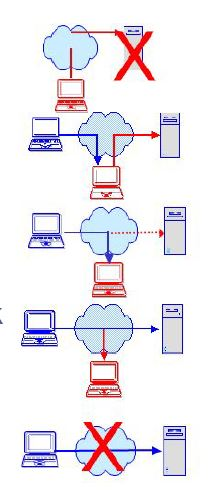
\includegraphics[scale = 0.8]{images/threatModel.JPG}
\end{center}
\end{multicols}


\section{Formální definice hašovacích funkcí, jaké jsou jejich požadované vlastnosti, jak se hodnotí jejich bezpečnost. Uveďte příklady použití hašovacích funkcí.}

Funkce, která z libovolně dlouhého vstupu M vytvoří výstup o konstantní délce.

Požadavky jsou jednocestnost (nelze z hashe vypočítat původní zprávu) a bezkoliznost (je těžké najít dvě zprávy, které by měly stejný hash)

Odolnost proti kolizím:
\begin{itemize}
    \item Kolize prvního řádu -- nalezení vzoru
    \item Kolize druhého řádu -- nalezení druhé zprávy, aby měly stejný hash jako první
    \item Odolnost proti kolizím -- nalezení dvou různých zpráv, aby měly stejný hash (neznáme ani 1 zprávu)
\end{itemize}

Použití -- digitální podpisy, kontrola integrity, pro uložení hesel, uložení klíčů, prokázání autorství\dots

\section{Vysvětlete princip konstrukce iteračních hašovacích funkcí, jaké jsou na ně kladené požadavky, jak se hodnotí jejich bezpečnost.}

Využívá speciální kompresní funkce \textit{f}, která bere vstup z předchozího kroku a kombinuje ho s n-bitovým blokem vstupní zprávy. Na poslední blok zprávy je použit padding. Na konec iterační šifry se přidává blok s délkou zprávy (damgar-merklovo zkreslení).

Je požadována rychlost a zároveň bezpečnost. Příklady MD5, sha1, sha2.

\section{Vysvětlete princip konstrukce hašovacích funkcí typu „houba“ (SHA3), příklady využití.}

\begin{enumerate}
    \item Upravíme vstup pomocí paddingu
    \item Absorbing -- Postupně se přidávají bloky ze vstupní zprávy (ty se xorují s bitovou rychlostí \textit{r}) Výsledek xorovaní a kapacita \textit{c} vstupuje do kompresní funkce (2 vstupy a 2 výstupy).
    \item Squezing -- slouží k získaní hashe. Ten je získán z \textit{r}.
\end{enumerate}

Vždy musí platit $r+c=1600$ s tím že už existují předdefinované hodnoty.

Využití je pro digitální podpis, integritu dat\dots

\section{Vysvětlete princip jednorázového podpisu pomocí hašovacích funkcí (Lamport), uveďte jeho výhody a nevýhody.}

Je to metoda pro konstrukci digitálního podpisu (podepisuje se každý bit zvlášť).
\begin{enumerate}
    \item Vygenerují se dvě sady náhodných řetězců a z obou se vytvoří hashe (budou dva sety hashu)
    \item Hashe se zveřejní a řetězce se uschovají.
    \item Podpis pokud je bit 0 zveřejní se hash prvního setu při 1 se zveřejní hash druhého setu
    \item Pro ověření se provede stejný postup a porovná se s přijatým podpisem
\end{enumerate}

Výhodou je, že pokud by byly Lampartovy podpisy s velkými hashovacími funkcemi tak nejsou ohroženy kvantovými počítači.

Nevýhodou je že každý klíč může být použit pouze k podepsání jedné zprávy.

\section{Vysvětlete princip jednorázového podpisu Winternitz, uveďte jeho výhody a nevýhody.}

\begin{enumerate}
    \item Vygeneruje se 32 256 bit náhodných hodnot (privátní klíč)
    \item Každá hodnota je hashována 256x a tím vzniknou veřejné klíče
    \item Vezme se zpráva a je hashována na 256bit
    \item Hash zprávy se rozdělí na 32 bloku
    \item Privátní klíč se hashuje 256-hodnota bloku zprávy
    \item Tímto vznikne podpis takže bude 32 256 bitových hodnot
\end{enumerate}

Ověření:
\begin{enumerate}
    \item Vezme se podpis rozdělí se na 32 bloků
    \item Každý blok se zahashuje o velikost bloku zprávy
    \item Výsledek je veřejný klíč
\end{enumerate}


\section{Jak souvisí hodnota entropie s bezpečností kryptografických generátorů náhodných čísel.}

Entropie určuje míru náhodnosti, jak je složité předvídat hodnotu. Entropie generátoru je maximální, pokud se pro danou délku generují všechny kombinace se stejnou pravděpodobností. Pokud by útočník dokázal s jistotou předpovídat hodnoty tak míra entropie je nulová.

\section{Jaké jsou požadavky kladené na kryptograficky bezpečné generátory náhodných čísel.}

\begin{itemize}
    \item Rovnoměrné rozložení -- jsou generovány se stejnou pravděpodobností
    \item Nezávislost hodnot
    \item Nepredikovatelnost -- next-bit test
    \item State compromise -- při zjištění vnitřního stavu generátoru, nelze vygenerovat původní hodnoty.
\end{itemize}

\section{Uveďte příklady realizace kryptograficky bezpečných generátorů náhodných čísel.}

\textbf{True random number generator} -- Založeno na nepredikovatelných fyzikálních procesech, například tepelný šum, radioaktivní rozpad.

\textbf{Pseudo random number generator} -- Jde složitě predikovat, kvůli velkému množství vstupů, například linux PRNG sběr událostí na PC (pohyb myši, HDD\dots), blum-blum-shub PRNG, LFSR (linear feedback shift registr)

\section{V čem spočívá hrozba využití „kvantových počítačů“ pro kryptografii, uveďte příklady.}

TODO

\section{Uveďte důvody použití kvantové distribuce klíčů (QKD). Jakým způsobem se u QKD informace přenáší, jaké jsou realizační problémy, popište princip protokolů BB84, EPR a COW. K čemu se využívá „kvantový přenos informace“. Uveďte důvody použití, příklady protokolů.}

\textbf{QKD} -- slouží jako náhrada asymetrického klíče. K přenosu se využívá fotonů v optickém vlákně.

\textbf{BB84} -- Neřeší autentizaci uživatelů a slouží k dohodě na symetrickém klíči. Je založen na principu neurčitosti ve spojení s polarizačním nebo fázovým kódováním.

\textbf{EPR} -- Využívá kvantově provázaný pár fotonů. Je vyžadována autentizace. Využívá se pro přenos v optických vláknech.

\textbf{COW} -- Bity se kódují do koherentních pulzů. Při odposlechu se bity jednoduše naruší.

\textbf{Kvantový přenos informace} --  Využití pro distribuci šifrovacího klíče, náhrada asymetrického systému.

\section{Vysvětlete, co je digitální podpis, jaké jsou na něho kladené požadavky a jakým způsobem se používá v součinnosti s hašovací funkcí.}

Digitální podpis je podpis vytvořen za pomoci kryptografických prostředků. Je založen na symetrických i asymetrických algoritmech. Má stejné požadavky jako ruční podpis (nezfalšovatelnost, nepřenosný, dokument nelze změnit, podpis nelze popřít). Digitální podpis je hash zašifrované zprávy soukromým klíčem podepisovatele. 

Můžeme podepisovat na přímo mezi dvěma subjekty nebo za pomoci třetí strany. 

\section{Vysvětlete, co je časové razítko, jakým způsobem se vytváří, jaké jsou na něho kladené požadavky.}

Slouží k potvrzení existence dokumentu v daném čase. Slouží k dlouhodobé archivaci elektronicky podepsaných dokumentů. 

Tvorba:
\begin{enumerate}
    \item Vytvoří se dokument k podepsání (hash)
    \item Ten se odešle autoritě časové značky
    \item Autorita přidá časovou značku
    \item Autorita tyto zašifruje společně hash a časovou značku svým privátním klíčem
    \item Odešle zpět žadateli podepsanou časovou značku
\end{enumerate}

Zdroj času musí být důvěryhodný tj. že musí být například synchronizován se třemi dalšími zdroji času, musí pocházet z důvěryhodného zdroje, nemůže se měnit.

\section{V souvislosti s nařízením eIDAS vysvětlete pojmy:}

\textbf{Elektronický podpis}-- Certifikáty pro potvrzení identity osob, serverů nebo webových stránek. Slouží pro elektronickou komunikaci.

\textbf{Zaručený elektronický podpis} -- Podpis se považuje za zaručení pokud poskytuje jedinečné identifikační údaje, kterého ho spojují s podepisující osobou.

\textbf{Kvalifikovaný elektronický podpis} -- Potvrzení o pravosti uznávaného elektronického podpisu, které bylo vydáno kvalifikovaným poskytovatel důvěryhodných služeb.

\textbf{Elektronická pečeť} -- Data v elektronické podobě, která jsou připojena k jiným datům v elektronické podobě nebo jsou s nimi logicky spojena s cílem zaručit původ a integritu.

\textbf{Elektronické časové razítko} -- Služba poskytována certifikační autoritou, umožnující prokázat daný dokument v čase.

\section{Znázorněte, popište princip činnosti asymetrického kryptosystému McEliece.}

Klíče:
\begin{itemize}
    \item S je k x k náhodná binární regulární matice
    \item G je k x n generující matice kódu C
    \item P je n x n náhodná binární permutační matice
    \item G' je k x n vypočtena jako SGP
\end{itemize}

Šifrování $c = m * G' + z$

Dešifrování $c' = c * P^{-1}$ poté $m' = D_c(c')$ nakonec $m = m' * S^{-1}$

\section{Znázorněte, popište princip činnosti asymetrického kryptosystému založeného na mřížkách, jaké „těžké“ matematické problémy se zde využívají, naznačte princip šifrování a dešifrování.}

Matematická struktura, která je použita k reprezentaci nekonečné mřížky bodů. Každá mřížka je tvořena vektory, které když spolu vynásobíme tak vytvoří jakýkoliv bod v mřížce. 

Problém nejkratšího vektoru -- Nalezení nejkratšího nenulového vektoru v mřížce z základu mřížky.

Problém nejbližšího vektoru -- Nalezení nejbližšího bodu (vektoru) v mřížce od zadaného bodu (vektoru)

\begin{enumerate}
    \item Vytvoříse se matice A.
    \item Alice vybere privátní x (vektor)
    \item Alice veřejný vektor $u = A*x$
    \item Bob vytvoří dva vektory b
    \item $b_1 = A*s + e_1$ kde $e_1$ a $s$ je náhodný soukromý vektor
    \item $b_2 = s* u + e_2 + m * \frac{9}{2}$
    \item dešifrování probíhá jako $b2 - b1 * x$
\end{enumerate}

\section{Asymetrický systém ECDH nad Fp: k čemu slouží, uveďte postup volby parametrů, výpočet klíčů, popis funkce systému.}

Slouží k vytvoření šifrovaného spojení a tvorbu symetrického šifrovacího klíče pro šifrování
zbytku komunikace. Výhoda je že využívají mnohem menší délku klíče 160b. Eliptická křivka \textit{E} je definována nad $F_p$ a P je bod na eliptické křivce, je generátor cyklické grupy.

\begin{table}[ht]
\centering
\begin{tabular}{lcl}
Alice && Bob \\
$k_{prvA} = a$ && $k_{prvB} = b$ \\
$k_{pubA} = A = a*P$ & $\stackrel{A}{\rightarrow}$ $\stackrel{B}{\leftarrow}$ & $k_{pubB} = B = b*P$ \\
$K_{AB} = a * B$ && $K_{AB} = b * A$ \\
\end{tabular}
\caption*{Znázornění ECDH výměny.}
\end{table}

\section{Popište Hastadův útok na systém RSA s malým veřejným exponentem.}

Zpráva \textit{m} byla zašifrována 3 různými klíči jako $c_i = m^3 \mod n_i$. Lze předpokládat že čísla \textit{n} jsou nesoudělná.

Ze šifrovaných textů $c_i$ lze vypočítat \textit{c}, jako $c \equiv c_i \mod n_i \Rightarrow m^3 \equiv c(\mod n_1n_2n_3)$. Jelikož $m < n_i$ je $m^3 < n_1n_2n_3$.

Otevřený text spočítáme jako $m = \sqrt[3]{c}$

\section{Slepý podpis na základě RSA: jak se vytváří, k čemu slouží?}

Autor a podepisující jsou různí s tím že podepisující nezná obsah zprávy. Pokud podepisující narazí na odtajněnou podepsanou zprávu, nesmí poznat, kdy a komu ji podepsal. Používá se k elektronickým volbám, elektronickým mincím. 

\begin{enumerate}
    \item Zvolíme náhodné číslo $r < n$
    \item Vytvoříme zaslepenou zprávu $m' = mr^e \mod n$
    \item Předáme $m'$ k podpisu a dostaneme $s' = m'^d \mod n$
    \item Spočítáme $s = s'r^{-1} \mod n$
    \item Platí $s = (mr^e)^dr^{-1}\equiv m^d \mod n$
\end{enumerate}

\section{Známe číslo c,z,m a hledáme číslo e v následujícím vztahu: \(c\equiv z^e (\mod m)\). O jaký matematický problém jde? Proč se jedná o matematický problém? O tento problém se opírá bezpečnost mnoha kryptografických systémů, uveďte alespoň jeden.}

Jedná se o problém diskrétního logaritmu. Například DH, elgamal, DSA. O problém se jedná jelikož je není nalezeno řešení v polynomiálním čase, takže pro velká čísla je výpočetně zdlouhavý (komplexita O($n^3$)).

\section{Jaký kryptografický systém se opírá o problém faktorizace? Popište problém faktorizace a uveďte příklad, jakým je faktorizace využita pro prolomení daného kryptografického systému.}

RSA. Jedná se o problém rozložení celého čísla na součin menších celých čísel. Lze využít například faktorizaci dělením nebo polárdův algoritmus.

\begin{enumerate}
    \item Vstup je n
    \item n dělíme postupně prvočísli menšími než $\sqrt{n}$
    \item Pokud je zbytek po dělení roven 0 našli jsme jeden z faktorů
    \item Výsledek po dělení dělíme znovu faktorem.
    \item Pokud je zbytek jiný než nula zkoušíme dalším faktorem.
\end{enumerate}

\section{K čemu lze FNF využít, hlavní výhody a nevýhody FNF, požadované vlastnosti FNF.}

K zamezení padělání nebo nedovolené manipulaci. Výstup je unikátní takže by šel použít ke generování čísel. Slouží jako alternativa ke klasickému bezpečnému ukládání tajných klíčů kryptosystémů.

\textbf{Výhody} -- Redukce nákladů, zvýšení úrovně zabezpečení (odolnost proti reverznímu inženýrství).

\textbf{Nevýhody} -- Šum ve výstupních odpovědích, je nutný nějaký korekční kód, možnost útoků postranními kanály.

Vlastnosti
\begin{itemize}
    \item Vytvořitelnost a vyhodnotitelnost
    \item Reprodukovatelnost
    \item Jedinečnost a identifikovatelenost
    \item Fyzická neklonovatelelnost
    \item Nepředvídatelnost
    \item Matematická a skutečná neklonovatelenost
    \item Jednocestnost
    \item Doložitelnost manipulace
\end{itemize}

\section{Uveďte tři typy FNF a popište, na jaké principu pracují.}
\textbf{Neelektronické} -- Fosforové FNF. Do materiálu nebo na povrch jsou přidávány částice fosforu. Lze detekovat pomocí UV a vyhodnocení probíhá optickým snímačem.

\textbf{Zpoždění elektrického obvodu} -- Povlakové FNF. Využívají měření náhodné kapacity dielektrických částic ochranné vrstvy integrovaného obvodu. 

\textbf{Bistabilní stavy} -- Flip-flop FNF. Využívá se bistabilních KO, které jsou řízeny hodinami. Resetový signál uvede obvod do neustáleného stavu a po ustálení mají KO náhodně nabyté logické hodnoty.

\section{Pomocí čeho lze ověřit identitu určité entity? Uveďte kritéria výběru autentizační metody.}

Identitu, lze vytvořit pomocí znalosti tajné informace, biometrické charakteristiky nebo FNF.

Kritéria výběru:
\begin{itemize}
    \item Četnost autentizace uživatele
    \item Počet uživatelů autentizačního systému
    \item Místo autentizace
    \item Věk a postavení autentizovaných uživatelů
    \item Bezpečnost autentizační metody
    \item Náklady
    \item Náročnost
    \item Mobilita autentizace
    \item Uživatelská přívětivost
\end{itemize}

\section{Na jakém principu pracují autentizační protokoly? Uveďte využívané proměnné parametry v autentizačních protokolech, útoky na autentizační protokoly.}

Pracují na principu výzva-odpověď. Mezi dvěma entitami nebo s využitím třetí důvěryhodné strany. Využívá náhodná čísla, sekvenční čísla nebo časová razítka.

\textbf{Proměnné} -- sekvenční číslo, časové razítko, náhodné číslo použité pouze jednou.

\textbf{Útoky} -- Replay attack, MitM, eavesdropping, DoS, desynchronizační útok, útok na přenesení vlastnických práv, útok zpětné zjistitelnosti, reflection, využití paralelního spojení, útok prolínáním.

\section{K čemu se využívá BAN logika, čím se zabývá? O jakou logiku se jedná?}

Ban logika se zabývá autentizačními protokoly na abstraktní úrovni. Využívá se k formálnímu ohodnocení bezpečnosti autentizačních protokolů. Jedná se o epistemickou a doxastickou logiku (zabývají se úvahami o znalosti a víře.) 

\section{Jaké otázky si klade BAN logika? Jaké objekty BAN logika rozlišuje?}

\begin{itemize}
    \item Čeho chce zkoumaný protokol dosáhnout?
    \item Potřebuje zkoumaný protokol více předpokladů než jiný protokol?
    \item Vykonává zkoumaný protokol cokoliv nepotřebného, jenž by moho být vypuštěno bez ohrožení bezpečnosti?
    \item Šifruje zkoumaný protokol něco, co by mohlo být zasláno v otevřené formě bez ohrožení bezpečnosti.
\end{itemize}

Rozlišuje -- účastníky, šifrovací klíče, logické formule (výroky).

\section{Uveďte a popište tři definované konstrukce v BAN logice. Uveďte a popište tři definovaná pravidla v BAN logice.}

\subsection{Konstrukce}

P věří X -- P může jednat jako kdyby bylo X pravdivé.

P vidí X -- P přijal zprávu obsahující X, jenž může přečíst a zopakovat

P vyslovil X -- P v určitém čase zaslal zprávu obsahující X. Není známo před jakou dobou.

\subsection{Pravidla}

Pravidlo jurisdikce -- Vyjadřuje, že pokud P věří, že Q má jurisdikci na X a P věří že X věří X tak poté P věří Q ohledně pravosti X.

Pravidlo důvěry k množině výroků -- P věří množině výroků, pokud věří každému jednotlivému výroku zvlášť.

Pravidlo novosti celého výroku -- Pokud část výroku je nová, poté celý výrok je nový. P věří že výrok je nový, pak věří že množina (X, Y) je nová.

\section{Uveďte jednotlivé kroky analýzy protokolů pomocí BAN logiky.}

\begin{enumerate}
    \item Z původního protokolu se odvodí idealizovaná verze protokolu.
    \item Sepíší se předpoklady ohledně počátečního stavu.
    \item Logické formule se připojí k jednotlivým výrokům protokolu, jako tvrzení o stavu systému po každém výroku.
    \item Logické výchozí předpoklady se aplikují na předpoklady a tvrzení za účelem zjištění toho, v co věří jednotlivé strany protokolu.
\end{enumerate}

\section{Rabinův kryptosystém, uveďte postup volby parametrů, výpočet klíčů, postup pro šifrování a dešifrování, výhody-nevýhody.}

\section{Asymetrický systém ECMQV: k čemu slouží, popis funkce systému, výhody.}

\section{Vysvětlete princip Schnorova identifikačního a podpisového schématu.}

\section{Uveďte ideový návrh kryptosystému:}
\subsection{Pro autentizaci uživatelů přistupujících vzdáleně k serverové aplikaci. Popište kryptografické služby, které systém musí zajišťovat, uveďte kryptografické algoritmy, které lze využít.}

\begin{itemize}
    \item Autentizaci, integritu dat, řízení přístupu
    \item Blokovou šifru a hash
\end{itemize}

\subsection{pro důvěrnou komunikaci mezi senzory a vzdáleným řídicím systémem. Uvažujte malý výpočetní výkon a také malý paměťový prostor u senzorů. Popište kryptografické služby, které systém musí zajišťovat, uveďte kryptografické algoritmy, které lze využít.}

\begin{itemize}
    \item Důvěrnost a integrita dat, autentizace
    \item Blokovou nebo proudovou šifru, záleží na množství dat
\end{itemize}

\subsection{zajišťující důvěrný přenos multimediálních dat v reálném čase, jednotlivé stanice mají dostateční výpočetní výkon a dostatečný paměťový prostor. Popište kryptografické služby, které systém musí zajišťovat, uveďte kryptografické algoritmy, které lze využít.}

\begin{itemize}
    \item Autentizaci, integritu dat
    \item Proudová šifra
\end{itemize}

\subsection{pro autentizaci senzorů k centrálnímu řídicímu systému využívající principu fyzicky neklonovatelných funkcí.}

\begin{itemize}
    \item Důvěrnost dat, autentizace (pomocí FNF)
    \item FNF
\end{itemize}

\subsection{pro generování klíčů pro šifry AES/ RSA.}

\begin{itemize}
    \item Integrita dat, řízení přístupu, autentizace
    \item Bezpečný generátor čísel
\end{itemize}

\subsection{pro elektronická volby, volič nesmí mít možnost volit opakovaně a jeho volba musí být anonymní.}

\begin{itemize}
    \item Autentizaci, důvěrnost dat, integritu dat, řízení přístupu
    \item slepý podpis, asymetrickou šifru (RSA)
\end{itemize}


\subsection{pro elektronickou komunikaci občanů se státní správou.}

\begin{itemize}
    \item Autentizaci, integritu dat, řízení přístupu
    \item Bloková šifra, hash
\end{itemize}

\subsection{zajišťující důvěrnou elektronickou komunikaci mezi bankou a její vzdálenou pobočkou.}

\begin{itemize}
    \item Autentizaci, důvěrnost dat, integritu dat
    \item Blokovou šifru
    \item Využití tunelování
\end{itemize}
